%\VignetteIndexEntry{An introduction to the package geoRglm}
%\VignetteDepends{}
%\VignetteKeywords{spatial}
%\VignettePackage{geoRglm}
\documentclass[12pt,a4paper]{article}
\usepackage[latin1]{inputenc}
\usepackage[dvips]{graphicx}
%\usepackage{psfig,epsfig,psfrag}
\usepackage{color,enumerate,longtable}
\usepackage{texnames,lastpage,verbatim,fancyvrb}
%% possible conflicts with Rd.sty
%\usepackage{url,html}
%\usepackage{heqn}
%\usepackage{amssymb,amsmath,amsfonts}
%
% Page size
%
%\usepackage{setspace,calc}
%\setlength{\voffset}{-1.5in}
%\setlength{\hoffset}{-1in}
%\setlength{\topmargin}{30mm}
%\setlength{\oddsidemargin}{40mm}
%\setlength{\textwidth}{210mm-10mm-\oddsidemargin}
%\setlength{\textheight}{297mm-10mm-\topmargin-\headheight-\headsep}
%
% Sweave settings
%
% Setting default size for \includegraphics 
% setting global defaults for figures: directory, names and sizes  
%%%%% \ SweaveOpts{prefix.string=figures/fig,width=4,height=4}

% emulating Sweave: Sweave style for R input code and output
\DefineVerbatimEnvironment{Rin}{Verbatim}{fontshape=sl}
\DefineVerbatimEnvironment{Rout}{Verbatim}{}
\newcommand{\Rcmd}[1]{\textsl{\texttt{#1}}}

% loading Defs from Rd.sty
%% [OFC: few changes coz of local pdflatex font problems]
%\newcommand{\strong}[1]{{\normalfont\fontseries{b}\selectfont #1}}
\newcommand{\strong}[1]{{\textbf{ #1}}}
\let\pkg=\strong
\newcommand{\code}[1]{\texttt{\small #1}}
%\newcommand{\R}{{\normalfont\textsf{R}}{}}
\newcommand{\R}{{\textsf{R}}{}}
\newcommand{\sQuote}[1]{`#1'}
\newcommand{\dQuote}[1]{``#1''}
\let\command=\code

\title{\pkg{geoRglm} : a package for  generalised linear spatial models
\\{\it introductory session}}
\author{Ole F. Christensen \& Paulo J. Ribeiro Jr.}
\date{Last update: \today}

\usepackage{/users/olefc/R/share/texmf/Sweave}
\begin{document}

\maketitle

%% Sweave settings for includegraphics default plot size (Sweave dafault is 0.8)  
%% notice this must be after begin{document}
%%% \setkeys{Gin}{width=0.9\textwidth}


The package \pkg{geoRglm} provides functions
for inference in generalised linear spatial models using the software \R.
This document illustrates some of the capabilities of the package.

We assume that the user has a substantial knowledge about geostatistics, is familar with the \pkg{geoR} package
(see the  introductory session for \pkg{geoR}), 
and has a basic knowledge about Markov chain Monte Carlo methods. We also encourage the reader to study the literature about generalised linear spatial models.
A list of books, articles and a short FAQ can be found here).

The objective of this page is to introduce the reader to the 
\pkg{geoRglm} commands and show how they can be used.
The commands used here are basic examples of the package handling, where we typically use default arguments for the function calls.
We encourage the user also to inspect other function arguments.

For further details on the functions included in \pkg{geoRglm}, we refer to the \pkg{geoRglm} documentation.

\section{STARTING A SESSION AND LOADING DATA}
After starting an \R{} session, we first load \pkg{geoR} and \pkg{geoRglm} with the commands:
\begin{Schunk}
\begin{Sinput}
> library(geoR)
> library(geoRglm)
\end{Sinput}
\end{Schunk}

If the installation directories for the packages are not the default locations for \R{} packages, type:
\begin{Rin}
  library(geoR, lib.loc = "PATH_TO_geoR")
  library(geoRglm, lib.loc = "PATH_TO_geoRglm")
\end{Rin}
where \verb+PATH_TO_geoR+ and \verb+PATH_TO_geoRglm+ are the paths to the directories where \pkg{geoR} and \pkg{geoRglm} are installed, respectively.
If the packages are correctly loaded the following messages will be displayed:
\begin{Schunk}
\begin{Soutput}
-------------------------------------------------
geoR - functions for geostatistical data analysis
geoR version 1.4-5 (2004-02-23) is now loaded
-------------------------------------------------
\end{Soutput}
\begin{Soutput}
-----------------------------------------------------------
geoRglm - a package for generalised linear spatial models
geoRglm version 0.7-12 (2004-03-20) is now loaded
-----------------------------------------------------------
\end{Soutput}
\end{Schunk}

Typically, data are stored as an object (a list) of class \code{"geodata"} (see the \pkg{geoR} introductory session 
for more details on this). For the data sets considered here, the object will sometimes include a vector \code{units.m} consisting 
of observation times (for the Poisson distribution) or numbers $N$ in $bi(N,p)$ (for the binomial distribution).

We use the data sets  \code{p50} and \code{rongelap} included in the \pkg{geoRglm} distribution for 
the examples presented in this document. These data sets can be loaded by typing:
\begin{Schunk}
\begin{Sinput}
> data(p50)
> data(rongelap)
\end{Sinput}
\end{Schunk}
Helpfiles are available for \pkg{geoRglm}. For getting help on the function \command{pois.krige}, just type:  
\begin{Rin}
> help(pois.krige)
\end{Rin}

\section{CONDITIONAL SIMULATION and SPATIAL PREDICTION}

Here we describe conditional simulation using MCMC and spatial prediction in the Poisson-log normal model,  when covariance parameters are fixed.
Full Bayesian methods are also implemented and will be presented in Section~3. 

The nugget effect parameter (microscale variation) in the underlying Gaussian field can be set to a fixed value. 
The same applies for the smoothness and anisotropy parameters. Options for taking covariates (trends) into 
account are also included.

Conditional simulation and prediction with fixed covariance parameters in the Poisson-log normal model can be performed 
with options for either fixed $\beta$ (OK) or flat prior on $\beta$ (SK).
The function uses a Langevin-Hastings MCMC algorithm for simulating from the conditional distribution.

An example where all parameters are fixed is shown below (for illustration purposes, some parameter values are just taken).  

First we need to tune the algorithm by scaling the proposal variance so that acceptance rate is approximately 60 percent (optimal
acceptance rate for Langevin-Hastings algorithm). This is done by trial and error. 
\begin{Schunk}
\begin{Sinput}
> model2 <- krige.glm.control(cov.pars = c(1, 1), beta = 1)
> test2.tune <- pois.krige(p50, krige = model2, mcmc.input = list(S.scale = 0.2, 
+     thin = 1))
\end{Sinput}
\end{Schunk}
After a few tryouts we decide to use \code{S.scale = 0.5}.
We also need to study how well the chain is mixing.
\setkeys{Gin}{width=0.8\textwidth}
\begin{figure}[h!]
\centering
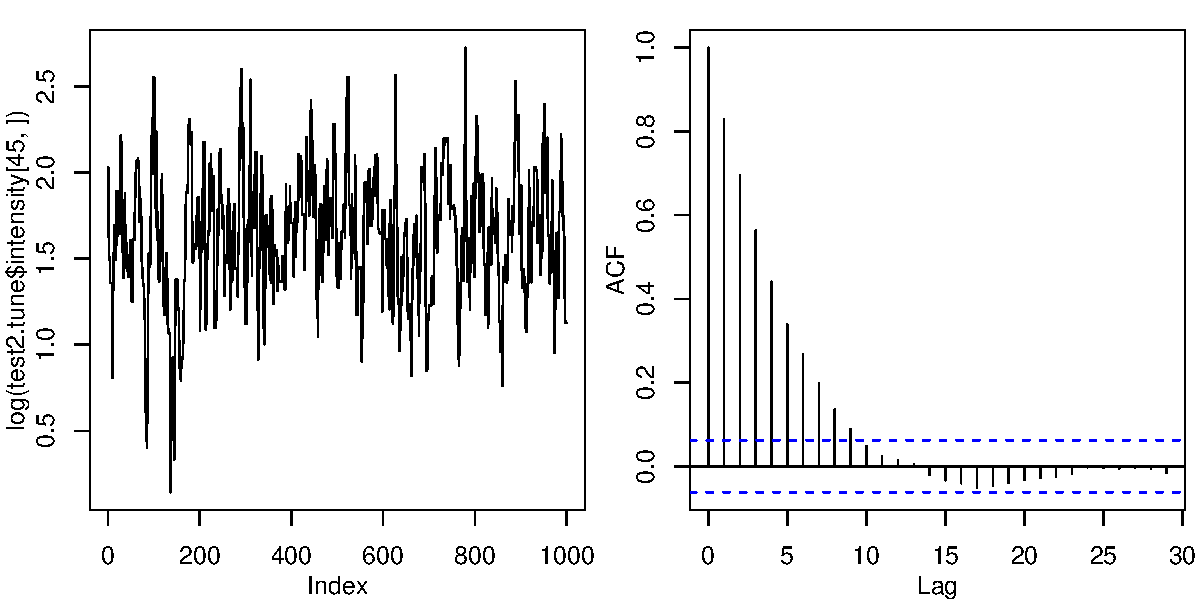
\includegraphics{geoRglmintro-006}
\label{fig:pois.krige}
\caption{Results from \texttt{pois.krige}.}
\end{figure}    
Here the functions in the \pkg{coda} package would be useful for assessing the convergence and inspect the mixing of the MCMC 
algorithm. For a small demonstration of a few CODA functions used on 
the output above, see here.

To reduce the autocorrelation of the samples we decide to subsample every 10 iterations (default); when working with real data sets we may need to make a more 
extensive subsampling, say, storing only every 1000 iterations.

Now we make (minimal mean square error) prediction of the intensity at the two locations (0.5, 0.5) and (1, 0.4).
\begin{Schunk}
\begin{Sinput}
> test2 <- pois.krige(p50, locations = cbind(c(0.5, 0.5), 
+     c(1, 0.4)), krige = model2, mcmc.input = mcmc.control(S.scale = 0.5), 
+     output = output.glm.control(sim.predict = TRUE))
\end{Sinput}
\end{Schunk}

The output is a list including the predicted values (\code{test2\$predict}), the prediction variances 
(\code{test2\$krige.var}) and the estimated Monte Carlo standard errors on the predicted values (\code{test2\$mcmc.error}). 
Please consider printing out the predicted values and the associated Monte Carlo standard errors:
\begin{Schunk}
\begin{Sinput}
> test2$predict
> test2$mcmc.error
\end{Sinput}
\end{Schunk}
Note that the Monte Carlo standard errors (the errors due to the MCMC-simulation) are small 
compared to predicted values, which is very satisfactory. (Monte Carlo standard errors on the prediction variances is not implemented yet).

By specifying \code{sim.predict = TRUE}, simulations are drawn from the predictive intensity at the two prediction locations (\code{test2\$simulations}). 
These simulations are plotted below. 
\setkeys{Gin}{width=0.8\textwidth}
\begin{figure}[h!]
\centering
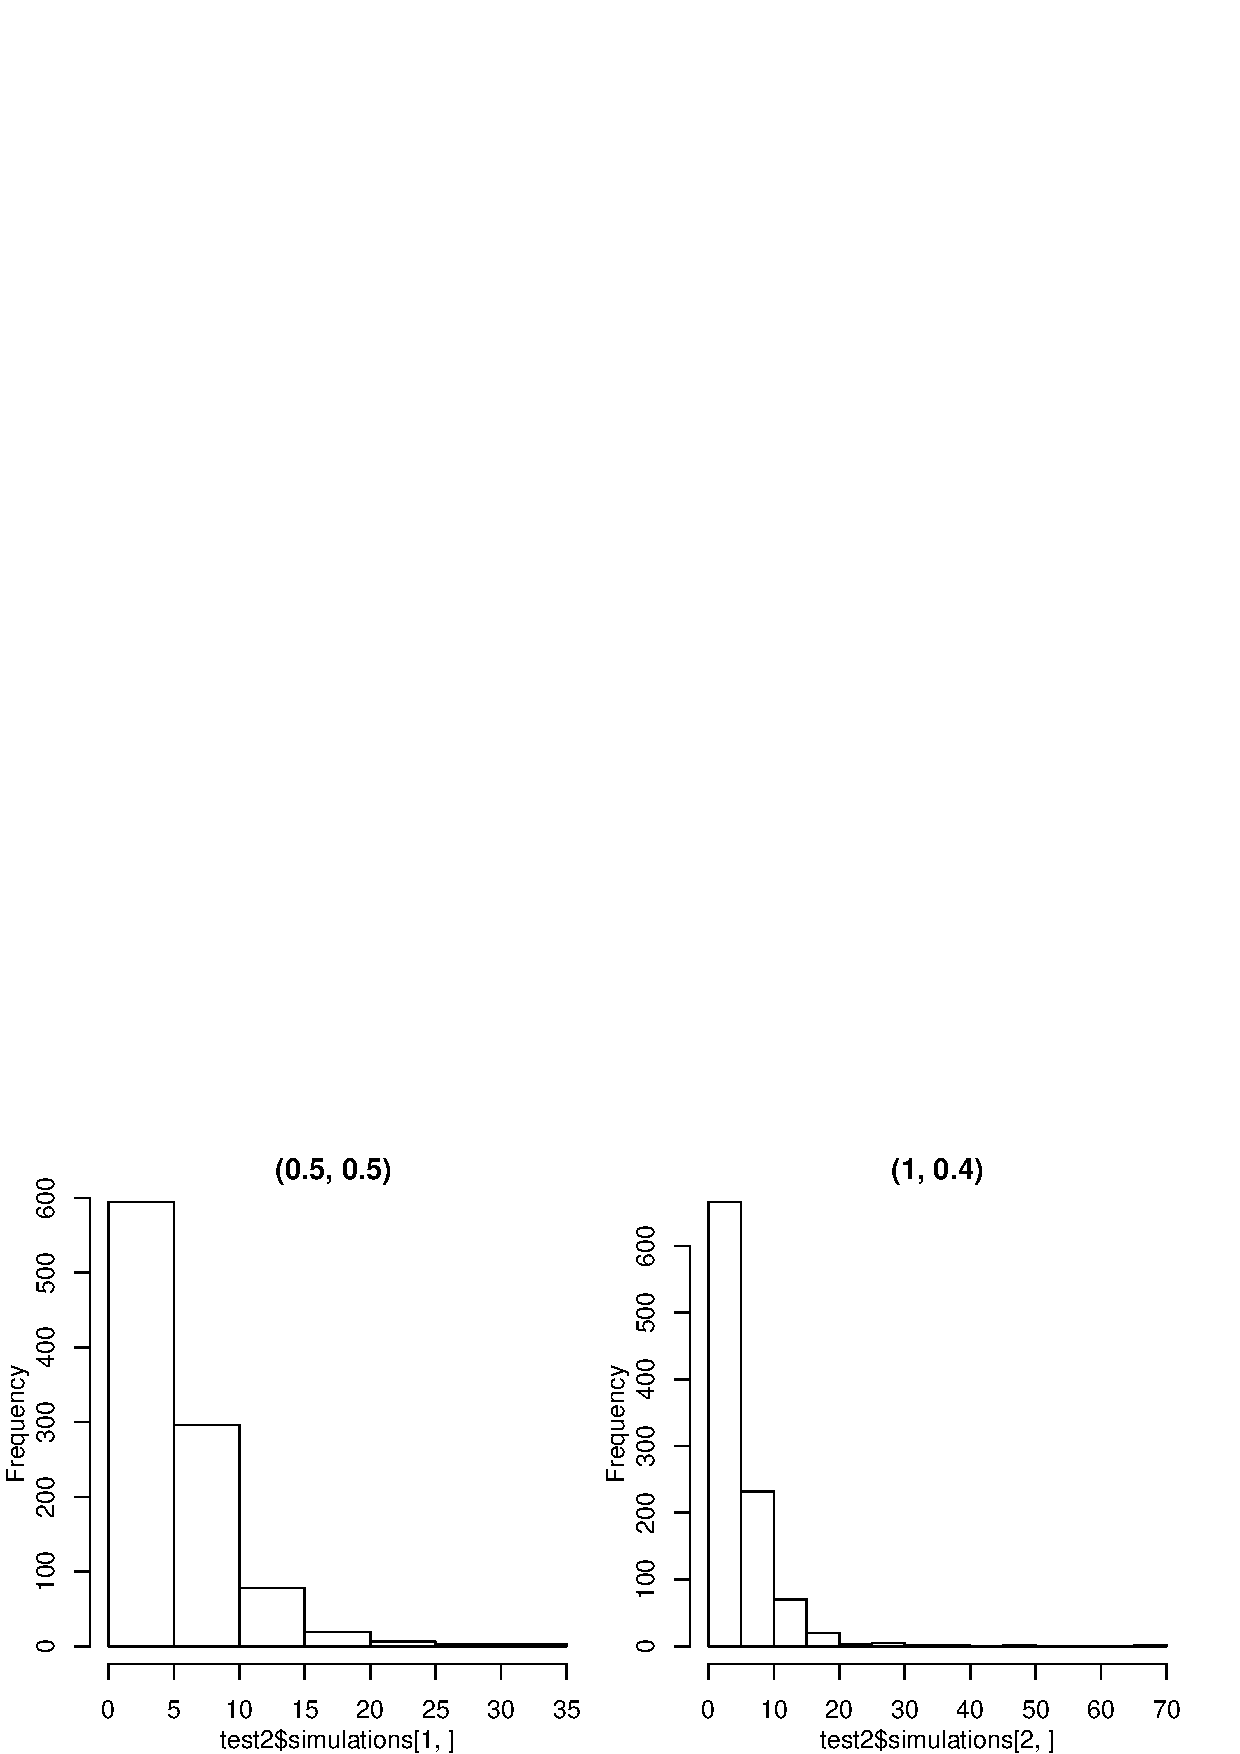
\includegraphics{geoRglmintro-009}
\label{fig:hist.sim.pk}
\caption{Histograms from 2 simulations.}
\end{figure}    

The way to specify that $\beta$ should follow a uniform prior would be:
\begin{Schunk}
\begin{Sinput}
> model2.u <- krige.glm.control(cov.pars = c(1, 1), beta = 1, 
+     type.krige = "ok")
> test2.unif.beta <- pois.krige(p50, krige = model2.u, 
+     mcmc.input = list(S.scale = 0.5))
\end{Sinput}
\end{Schunk}

\section{BAYESIAN ANALYSIS }

Bayesian analysis for the Poisson-log normal model and the binomial-logit model is implemented by the functions 
\command{pois.krige.bayes} and \command{binom.krige.bayes}, respectively.
Model parameters can be treated as fixed or random.        

As an example consider first a model without nugget and including uncertainty in the $\beta$ and $\sigma^2$ parameters (mean and variance of the random effects $S$, respectively). 
A Bayesian analysis is made by typing commands like: 
\begin{Schunk}
\begin{Sinput}
> prior5 <- prior.glm.control(phi.prior = "fixed", phi = 0.1)
> mcmc5.tune <- mcmc.control(S.scale = 0.01, thin = 1)
> test5.tune <- pois.krige.bayes(p50, prior = prior5, mcmc.input = mcmc5.tune)
\end{Sinput}
\end{Schunk}

Now chose \code{S.scale} (Acc-rate=0.60 is preferable).  
After having adjusted the parameters for the MCMC algorithm and checking the output we run an analysis.
%% PJ to Ole: notice the next generate a long output with mcmc status messages.
%% I've done a trick to avoid it to be printed
\begin{Schunk}
\begin{Sinput}
> mcmc5 <- mcmc.control(S.scale = 0.075, thin = 100)
> test5 <- pois.krige.bayes(p50, locations = t(cbind(c(2.5, 
+     3), c(-6050, -3270))), prior = prior5, mcmc.input = mcmc5, 
+     output = list(threshold = 10, quantile = c(0.05, 
+         0.99)))
\end{Sinput}
\end{Schunk}
\begin{Schunk}
\begin{Soutput}
pois.krige.bayes: model with mean being constant
iter. numb. 1000 ; Acc.-rate = 0.67 
iter. numb. 2000 ; Acc.-rate = 0.67 
iter. numb. 3000 ; Acc.-rate = 0.64 
iter. numb. 4000 ; Acc.-rate = 0.64 
iter. numb. 5000 ; Acc.-rate = 0.63 
iter. numb. 6000 ; Acc.-rate = 0.62 
iter. numb. 7000 ; Acc.-rate = 0.64 
iter. numb. 8000 ; Acc.-rate = 0.65 
iter. numb. 9000 ; Acc.-rate = 0.66 
iter. numb. 10000 ; Acc.-rate = 0.60 
iter. numb. 11000 ; Acc.-rate = 0.64 
iter. numb. 12000 ; Acc.-rate = 0.67 
iter. numb. 13000 ; Acc.-rate = 0.65 
iter. numb. 14000 ; Acc.-rate = 0.65 
iter. numb. 15000 ; Acc.-rate = 0.65 
iter. numb. 16000 ; Acc.-rate = 0.66 
iter. numb. 17000 ; Acc.-rate = 0.66 
iter. numb. 18000 ; Acc.-rate = 0.66 
iter. numb. 19000 ; Acc.-rate = 0.66 
iter. numb. 20000 ; Acc.-rate = 0.64 
iter. numb. 21000 ; Acc.-rate = 0.65 
iter. numb. 22000 ; Acc.-rate = 0.65 
iter. numb. 23000 ; Acc.-rate = 0.61 
iter. numb. 24000 ; Acc.-rate = 0.67 
iter. numb. 25000 ; Acc.-rate = 0.66 
iter. numb. 26000 ; Acc.-rate = 0.65 
iter. numb. 27000 ; Acc.-rate = 0.63 
iter. numb. 28000 ; Acc.-rate = 0.67 
iter. numb. 29000 ; Acc.-rate = 0.63 
iter. numb. 30000 ; Acc.-rate = 0.63 
iter. numb. 31000 ; Acc.-rate = 0.65 
iter. numb. 32000 ; Acc.-rate = 0.65 
iter. numb. 33000 ; Acc.-rate = 0.63 
iter. numb. 34000 ; Acc.-rate = 0.63 
iter. numb. 35000 ; Acc.-rate = 0.61 
iter. numb. 36000 ; Acc.-rate = 0.63 
iter. numb. 37000 ; Acc.-rate = 0.66 
iter. numb. 38000 ; Acc.-rate = 0.67 
iter. numb. 39000 ; Acc.-rate = 0.64 
iter. numb. 40000 ; Acc.-rate = 0.63 
iter. numb. 41000 ; Acc.-rate = 0.63 
iter. numb. 42000 ; Acc.-rate = 0.66 
iter. numb. 43000 ; Acc.-rate = 0.63 
iter. numb. 44000 ; Acc.-rate = 0.66 
iter. numb. 45000 ; Acc.-rate = 0.64 
iter. numb. 46000 ; Acc.-rate = 0.67 
iter. numb. 47000 ; Acc.-rate = 0.64 
iter. numb. 48000 ; Acc.-rate = 0.64 
iter. numb. 49000 ; Acc.-rate = 0.65 
iter. numb. 50000 ; Acc.-rate = 0.66 
iter. numb. 51000 ; Acc.-rate = 0.65 
iter. numb. 52000 ; Acc.-rate = 0.61 
iter. numb. 53000 ; Acc.-rate = 0.65 
iter. numb. 54000 ; Acc.-rate = 0.69 
iter. numb. 55000 ; Acc.-rate = 0.64 
iter. numb. 56000 ; Acc.-rate = 0.64 
iter. numb. 57000 ; Acc.-rate = 0.61 
iter. numb. 58000 ; Acc.-rate = 0.61 
iter. numb. 59000 ; Acc.-rate = 0.63 
iter. numb. 60000 ; Acc.-rate = 0.64 
iter. numb. 61000 ; Acc.-rate = 0.64 
iter. numb. 62000 ; Acc.-rate = 0.66 
iter. numb. 63000 ; Acc.-rate = 0.65 
iter. numb. 64000 ; Acc.-rate = 0.65 
iter. numb. 65000 ; Acc.-rate = 0.65 
iter. numb. 66000 ; Acc.-rate = 0.63 
iter. numb. 67000 ; Acc.-rate = 0.63 
iter. numb. 68000 ; Acc.-rate = 0.60 
iter. numb. 69000 ; Acc.-rate = 0.62 
iter. numb. 70000 ; Acc.-rate = 0.64 
iter. numb. 71000 ; Acc.-rate = 0.64 
iter. numb. 72000 ; Acc.-rate = 0.62 
iter. numb. 73000 ; Acc.-rate = 0.64 
iter. numb. 74000 ; Acc.-rate = 0.65 
iter. numb. 75000 ; Acc.-rate = 0.62 
iter. numb. 76000 ; Acc.-rate = 0.66 
iter. numb. 77000 ; Acc.-rate = 0.63 
iter. numb. 78000 ; Acc.-rate = 0.65 
iter. numb. 79000 ; Acc.-rate = 0.63 
iter. numb. 80000 ; Acc.-rate = 0.65 
iter. numb. 81000 ; Acc.-rate = 0.66 
iter. numb. 82000 ; Acc.-rate = 0.65 
iter. numb. 83000 ; Acc.-rate = 0.64 
iter. numb. 84000 ; Acc.-rate = 0.64 
iter. numb. 85000 ; Acc.-rate = 0.62 
iter. numb. 86000 ; Acc.-rate = 0.65 
iter. numb. 87000 ; Acc.-rate = 0.62 
iter. numb. 88000 ; Acc.-rate = 0.62 
iter. numb. 89000 ; Acc.-rate = 0.61 
iter. numb. 90000 ; Acc.-rate = 0.66 
iter. numb. 91000 ; Acc.-rate = 0.64 
iter. numb. 92000 ; Acc.-rate = 0.64 
iter. numb. 93000 ; Acc.-rate = 0.65 
iter. numb. 94000 ; Acc.-rate = 0.65 
iter. numb. 95000 ; Acc.-rate = 0.68 
iter. numb. 96000 ; Acc.-rate = 0.65 
iter. numb. 97000 ; Acc.-rate = 0.65 
iter. numb. 98000 ; Acc.-rate = 0.62 
iter. numb. 99000 ; Acc.-rate = 0.64 
iter. numb. 100000 ; Acc.-rate = 0.62 
MCMC performed: n.iter. =  1e+05 ; thinning =  100 ; burn.in =  0 
pois.krige.bayes: Prediction performed 
pois.krige.bayes: done!
\end{Soutput}
\end{Schunk}

The output is a list which contains the five arguments \code{posterior}, \code{predictive}, \code{model}, \code{prior} and \code{mcmc.input}. 
The \code{posterior} contains information
on the posterior distribution of the parameters, and the conditional simulations of the signal 
$g^{-1}(S)$ at the data locations. 
The \code{predictive} contains information on the predictions, where 
\code{predictive\$median} is the predicted signal and \code{predictive\$uncertainty} is the associated uncertainty.
The \code{threshold = 10} argument gives probabilities of the predictive distribution of the signal being less 
than 10 (\code{test5\$predictive\$probability}).
The \code{quantiles = c(0.05,0.99)} gives the 0.05 and 0.99 quantiles of the predictive distribution of the signal 
(\code{test5\$predictive\$quantiles}).

Below we show the simulations from the posterior distribution of the signal at a few data locations.
\setkeys{Gin}{width=\textwidth}
\begin{figure}[h!]
\centering
\includegraphics{geoRglmintro-014}
\label{fig:hist.sim.bayes}
\caption{Histograms}
\end{figure}

Now we consider an example with a random correlation scale parameter phi and a positive nugget for the random effects S. The program is using a discretised prior fpr phi, where the discretisation is given by
the argument \code{phi.discrete}). The argument \code{tausq.rel = 0.05} gives the relative nugget for S, i.e. the relative 
microscale variation.
\begin{Schunk}
\begin{Sinput}
> mcmc6.tune <- mcmc.control(S.scale = 0.075, n.iter = 2000, 
+     thin = 100, phi.scale = 0.01)
> prior6 <- prior.glm.control(phi.prior = "uniform", phi.discrete = seq(0.02, 
+     1, 0.02), tausq.rel = 0.05)
> test6.tune <- pois.krige.bayes(p50, prior = prior6, mcmc.input = mcmc6.tune)
\end{Sinput}
\end{Schunk}

Acc-rate=0.60 , acc-rate-phi = 0.25-0.30  are preferable. 
After having adjusted the parameters for the MCMC algorithm and checking the output we run an analysis.\\
\strong{WARNING: RUNNING THE NEXT COMMAND CAN BE TIME-CONSUMING}
\begin{Schunk}
\begin{Sinput}
> mcmc6 <- mcmc.control(S.scale = 0.075, n.iter = 4e+05, 
+     thin = 200, burn.in = 5000, phi.scale = 0.12, phi.start = 0.5)
> test6 <- pois.krige.bayes(p50, locations = t(cbind(c(2.5, 
+     3.5), c(-60, -37))), prior = prior6, mcmc.input = mcmc6)
\end{Sinput}
\end{Schunk}

Below we show the posterior distribution of the two covariance parameters and the beta parameter.
\setkeys{Gin}{width=\textwidth}
\begin{figure}[h!]
\centering
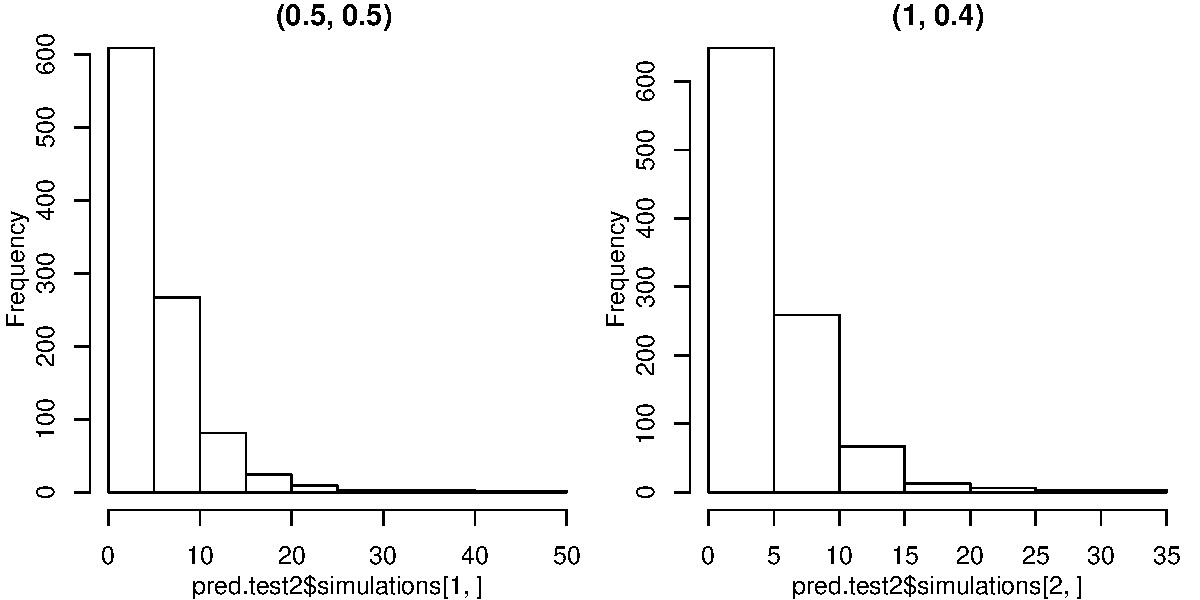
\includegraphics{geoRglmintro-017}
\label{fig:posterior}
\caption{Samples from the posterior}
\end{figure}

To calculate the Monte Carlo standard errors on the posterior means of the parameters, we use the function 
\code{asympvar}.
\begin{Schunk}
\begin{Sinput}
> sqrt(asympvar(test6$posterior$beta$sample)/2000)
\end{Sinput}
\begin{Soutput}
[1] 0.004044618
\end{Soutput}
\begin{Sinput}
> sqrt(asympvar(test6$posterior$sigmasq$sample)/2000)
\end{Sinput}
\begin{Soutput}
[1] 0.006110709
\end{Soutput}
\begin{Sinput}
> sqrt(asympvar(test6$posterior$phi$sample)/2000)
\end{Sinput}
\begin{Soutput}
[1] 0.004633281
\end{Soutput}
\begin{Sinput}
> sqrt(asympvar(log(test6$posterior$simulations))/2000)
\end{Sinput}
\begin{Soutput}
 [1] 0.010251472 0.012857275 0.011335576 0.014272616 0.015905545
 [6] 0.012096571 0.013930179 0.012385419 0.005964200 0.008644862
[11] 0.006228193 0.013724528 0.015421052 0.013761430 0.009418635
[16] 0.009246115 0.005926357 0.016600850 0.013414592 0.009735895
[21] 0.009850077 0.009136813 0.009583265 0.008635842 0.005453478
[26] 0.014913459 0.009043357 0.010115974 0.007419523 0.008163207
[31] 0.009370546 0.011980031 0.011487674 0.012426885 0.014113085
[36] 0.009426728 0.013041502 0.011040078 0.014049159 0.012780685
[41] 0.012166682 0.007473775 0.013803047 0.012190057 0.009141520
[46] 0.005409696 0.016415075 0.013819733 0.012634068 0.010307191
\end{Soutput}
\end{Schunk}

\paragraph*{Exercise}

Construct similar commands using \command{binom.krige.bayes} on the data set \code{b50} yourself
(you load the data set by typing \Rcmd{data(b50)}). 

\section{SIMULATION of a GENERALISED LINEAR SPATIAL MODEL}

The \pkg{geoR} function \command{grf} generates a simulation from a Gaussian random field. This function can be used to generate
a simulation from a generalised linear spatial model as follows.
\begin{Schunk}
\begin{Sinput}
> sim <- grf(grid = expand.grid(x = seq(1, 10, l = 10), 
+     y = seq(1, 10, l = 10)), cov.pars = c(0.1, 0.2))
> attr(sim, "class") <- "geodata"
> sim$units.m <- c(rep(1, 50), rep(5, 50))
> sim$data <- rpois(100, lambda = sim$units.m * exp(sim$data))
\end{Sinput}
\end{Schunk}
\setkeys{Gin}{width=0.5\textwidth}
\begin{figure}
\centering
\begin{Schunk}
\begin{Sinput}
> plot(sim$coords[, 1], sim$coords[, 2], type = "n")
> text(sim$coords[, 1], sim$coords[, 2], format(sim$data))
\end{Sinput}
\end{Schunk}
\includegraphics{geoRglmintro-020}
\label{fig:simulation}
\caption{Simulated data}
\end{figure}
Observe that the upper part of the figure corresponds to observation times equal to 5.
Therefore the simulated counts are larger.

\paragraph*{Exercise}

Generate a simulation from a spatial binomial random field. 

\section{ADDITIONAL INFORMATION }  

\begin{enumerate}   
\item  Empirical covariogram for the Poisson-log normal model. See here.  
  
\item  A short demonstration shown at my Ph.D. viva is found here. 
  
\item  The commands from the example in Diggle, Ribeiro Jr and Christensen (2003) [{\it bookchapter}], and Christensen and Ribeiro Jr (2002) [{\it R-news}] are found here.  
\end{enumerate}

\end{document}
